\documentclass{llncs}
\usepackage{makeidx, graphicx}
\begin{document}

\mainmatter
\title{Random Forest for the Real Forests}
\titlerunning{Forest Classification} 
\author{Sharan Agrawal\inst{1} \and Shivam Rana\inst{2} \and Tanvir Ahmad\inst{3}}
\authorrunning{Sharan Agrawal et al.}
\tocauthor{Sharan Agrawal, Shivam Rana, Tanvir Ahmad}


\institute{Dept. of Computer Engineering, Jamia Millia Islamia, Delhi, India,\\
\email{\inst{1}sharan.agrawal@outlook.com, \inst{2}shivamrana95@yahoo.in, \inst{3}tahmad2@jmi.ac.in}}

\maketitle

\begin{abstract}
A forest is a vast area of land covered predominantly with trees and undergrowth. In this paper, adhering to cartographic variables, we try to predict the predominant kind of tree cover of a forest using the Random Forests (RF) classification method. The study classifies the data into 7 classes of forests found in the Roosevelt National Forest of Northern Colorado. With sufficient data to create a classification model RF classifier gives reasonably accurate results. Fine tuning of the algorithm parameters was done to get promising results. Besides that a dimensionality check on the data set was conducted to observe the possibilities of dimensionality reduction.
\keywords{Random Forests, Dimensionality Reduction, Forest's Classification}
\end{abstract}


\section{Introduction}

Forests are one of the most extensive terrestrial ecosystems on Earth, and are widespread around the globe. The influence of forests and humans on each other has been observed to be both favorable as well as critical. Forests provide a vast array of services but, along with those they also bring environmental, economic, health and aesthetic costs. Thus, it is beneficial for us to observe the cover-type of forests which tells us about the predominant kind of tree cover, expanse of forests, ecosystems, and features such as carbon stocks.

Among many classification algorithms considered for our research Random Forests (RF) proved to be the most accurate, a classification algorithm which constructs a large number of decision trees at training time (called an ensemble) and gives the mode or mean prediction(regression) of individual trees as the output. RF basically gives a method to find the average prediction of a multitude of decision trees, which have been constructed on the basis of different instances (cross-validation) from the same data set\cite{StatLearn}. This leads to a minor loss in interpretation ability, but generally results in a stable model.

Accuracy of classification was boosted by dimension reduction techniques. Dimension represents the number of random variables (or the number of attributes) present in our data-set. In statistics, the method of reduction of the number of random variables in consideration is known as dimensionality reduction. As dimensionality increases, the data increasingly becomes more sparse which is problematic from a statistical point of view. Prediction becomes difficult in case of high-dimensional data as a colossal amount of training data is required to ensure that there are significant number of samples with each combination of values and unavailability of such a training data leads to a loss in predictive power (also known as the Hughes effect\cite{hughes}). Another technique used in our research for boosting the accuracy of our result was Cross-Validation, which is basically an iterative testing method usually influential with large data-sets, in which the same algorithm is applied multiple times selecting different instances of the data. The average of the classifications is then considered as the final prediction.

\section{Related Works}

The development of algorithm for RF was influenced by the work of Amit and German\cite{AmitGer} in 1997 who introduced the idea of searching over a randomly selected subset of the available decisions when splitting a node, in order to construct a single tree. This idea was evolved into RF by Breiman\cite{Breiman}. RF has been used in variegated fields such as network intrusion detection\cite{ZhangZulker}, fraud detection in online retailing\cite{AltenBren}, Patient Response prediction\cite{DittKhosh}, Cancer Classification\cite{Srivastava} and image data classification\cite{Boinee} because of its robustness to noise and the accuracy of its predictions. Geng, Cosman, Berry, Feng, and Schafer\cite{Geng} used RF classifier to identify the type of worm by analyzing it's body movements. In a 2006 experiment by Diaz-Uriarte and Alvarez de Andres, RF classifier was used on ten different DNA micro-array data-sets procured from a variety of diseases which affect humans\cite{DiazAlvarez}. They found that, RF is competitive with alternative methods, without the necessity of any fine-tuning of parameters or pre-selection of variables. RF classifier also performs fairly accurately in pattern recognition concerning the diagnosis of Gas Turbine blading faults\cite{Margou}. In this research, randomness was introduced to the trees in two different ways, based on different theoretical assumptions. The classifier was then compared against other Machine Learning algorithms such as Neural Networks, Classification and Regression Trees, Naive Bayes and K-Nearest Neighbor. Accuracy of 97\% was achieved in terms of precision and recall, which was an enhancement to the existing levels accomplished by Neural Networks by a factor of 1.5\%-2\%.

Dimensionality Reduction (DR) is also an important technique in data mining. DR methods have been used to deal with the Curse of Dimensionality in case of analysis of a wide variety of data\cite{HuZahorian}\cite{Bostrom}.


\section{Proposed Architecture}

Figure \ref{framework} describes the proposed methodology we employed for the classification of forests based on the forest cover type, having following modules - Data Preprocessing, Accuracy based Classifier Selection, Classifier and Dimensionality Reduction.

\begin{figure}
  \centering
    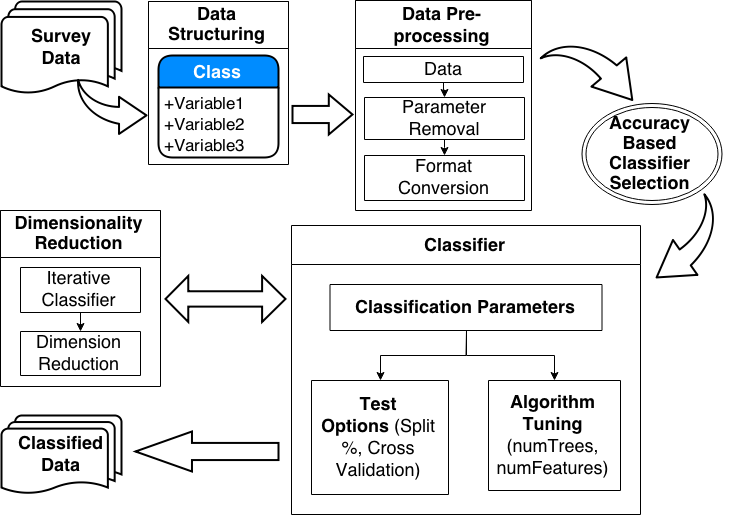
\includegraphics[width=\textwidth]{framework.png}
  \caption{Proposed Architecture of Classification}
  \label{framework}
\end{figure}

\subsection{Procuring the Data-set}

This is the primary step during which data obtained from the surveys are used to derive the independent variables. A raw (not scaled) data set is obtained and saved in a standard format (eg. CSV).

\subsection{Data Pre-processing}
Various data pre-processing steps like data scaling, field removal and format conversion were applied that can be summarized as follows. In the field removal steps columns like ID, Serial No. are removed from the data since these columns are used for identifying the rows and have no role in classification.

\subsection{Accuracy based Classifier Selection}
In this step the emphasis is on the selection of the classification algorithm. The data set should be tried on various Machine learning (ML) algorithms. The classifier with highest accuracy is selected as the base learner.

\subsection{Classifier}
An algorithm that implements classification that is grouping of the data, is known as a classifier. The algorithm selected in the previous step is further experimented with in this step using the concepts like bootstrapping, random feature selection. Further, various parameters of the classifier are tuned to get more accurate results.

In order to tune the classification a number of options such as cross-validation (CV), \% split of data-set were used with the objective of producing the best possible results with a model built upon the training set. Cross validation is usually preferred over \% split as it brings a level of randomness in the classification. Cross Validation's one round involves splitting a sample of data into complementary subsets, training being done with a subset (training set) and testing  on other subset (testing set). To reduce variability, the validation results of multiple rounds of CV are averaged over the total rounds. The parameters that affect the performance of the classifier are recognized and manipulated to get an optimum (both time and accuracy) level.

\subsection{Dimension Reduction (DR)}
DR is the process of removal of variables from the data set which are correlated with each other and might degrade the classifier accuracy. Following steps were performed in order to improve the accuracy.

\subsubsection{Iterative Classification}

Each variable in the data set is excluded one by one and a model is built using the RF Classifier, variables whose exclusion results in accuracy higher than the default accuracy (when no variable is removed) are noted down.

\subsubsection{Dimension Reduction}

Candidate variables are chosen out of the variables obtained in the previous step, such that, their removal does not affect the accuracy of classification model. Among those candidates for the pair about which we have a rationale for their removal are removed. This accuracy driven DR approach is also known as the ’wrapper’ approach.


\section{Experimental Setup}

The experimental setup for our research was divided into the following modules:

\subsection{Experimental Data-set}

Our data-set contains following 54 strictly cartographic variables - Elevation, Aspect, Slope, Horizontal Distance To Hydrology, Vertical Distance To Hydrology, Horizontal Distance To Roadways, Hill-shade 9am (Hill9), Hill-shade Noon (HillNoon), Hill-shade 3pm (Hill3), Horizontal Distance To Fire Points, Wilderness Area (4 binary factors, 1 = presence \& 0 = absence), Soil Type (40 binary factors, 1 = presence \& 0 = absence). There were a total of 15210 rows of observations distributed equally (2160 instances each) among 7 classes of forests namely, Spruce/Fir, Lodgepole Pine, Ponderosa Pine, Cottonwood/Willow, Aspen, Douglas-fir, Krummholz.


\subsection{Data Pre-processing}

Weka\footnote{http://www.cs.waikato.ac.nz/ml/weka/} which is a data mining software in Java. The raw training data-set procured by us (in csv format) was converted to a format which Weka can recognize. The 'Id' field was also excluded for the facilitation of further processing.

\subsection{Accuracy based Classifier Selection}

\begin{table}[!t]
    \renewcommand{\arraystretch}{1.2}
    \caption{Accuracy with various Classifiers}
    \label{classifier}
    \centering
        \begin{tabular}{|c|l|c|}
        \hline\rule{0pt}{12pt}
        \textbf{SNo.} & \textbf{Algorithm} & \textbf{Accuracy} \\[2pt]
        %  & & \\
        \hline
        1 & Naive Bayes & 65.7804 \\ \hline
        2 & Decision Table & 69.3519 \\ \hline
        3 & Bayesian Belief Network & 69.6825 \\ \hline
        4 & Random Tree & 74.5833 \\ \hline
        5 & Classification via Regression & 80.3638 \\ \hline
        6 & J48 & 80.7606 \\ \hline
        7 & Bagging & 82.7315 \\ \hline
        8 & Random Forest & 87.0643 \\ \hline
        \end{tabular}
\end{table}


Many ML algorithms used for this step have already been implemented in Weka and applied upon the training data set using the software's GUI. The summarized results of accuracies for various ML algorithms in table \ref{classifier} shows that the RF classifier being most accurate (87.06 \% accuracy), should be the obvious choice.

\subsection{Random Forest Classifier}
RF is a classification algorithm which constructs a large number of trees (called an ensemble) at training time and gives the mode or mean prediction (regression) of the individual trees as the output. The robustness of the RF classifier was improved by using bootstrapping and random selection of attributes in the tree construction process. A diverse collection of robust trees lowers the overall classification error rate and enhances the effective solidity of the classifier. The classifier further undergoes the following two steps.

\subsubsection{Test Options}

Out of two test options cross-validation (CV) and \% split we preferred CV with 10 folds as discussed in section 3.


\subsubsection{Algorithm Tuning}
RF Classifier works mainly on two factors viz. numTrees (number of trees to be used to build the model) and numFeatures (randomly selected number of attributes to be considered at each node when building the trees). The preferable\cite{Khoshgoftar} values for the above two factors (numTrees, numFeatures) are 100 trees and M/3 features ('M' represents the total number of attributes). The modification of parameters was done using Weka GUI in the algorithm options.


\subsection{Dimensionality Reduction}

As stated in the Proposed Architecture (Section 3) here we used Iterative Classification and Dimension Reduction processes to reduce the dimensionality of the data. In our data-set, there a correlation was observed between variables Slope and Aspect and also between all the hill-shades (Hill9, HillNoon, Hill3). Based on the analysis of the data and the accuracies obtained after the removal of various combinations of the above correlated fields (as summarised in the table \ref{accuracy}), we decided to remove slope, Hill9 and Hill3 from the data. The rationale of their removal has been discussed in the next section (Section 5).


\begin{table}[!t]
    \renewcommand{\arraystretch}{1.2}
    \caption{Result}
    \label{accuracy}
    \centering
        \begin{tabular}{|c|c|c|}
        \hline\rule{0pt}{12pt}
        \textbf{Sno.} & \textbf{Features Excluded} & \textbf{Accuracy} \\[2pt]
        \hline
        1 & None & 87.064 \\
        \hline
        2 & Hill-shade at 3PM & 87.368 \\
        \hline
        3 & Hill-shade at 9AM & 87.262 \\
        \hline
        4 & Hill-shade at Noon & 87.050 \\
        \hline
        5 & Slope & 87.209 \\
        \hline
        6 & Aspect & 87.202 \\
        \hline
        7 & Elevation & 83.691 \\
        \hline
        8 & Aspect, Hill-shade at 9AM, Hill-shade at 3PM & 87.652 \\
        \hline
        9 & Aspect, Hill-shade at Noon, Hill-shade at 3PM & 87.341 \\
        \hline
        10 & Aspect, Hill-shade at 9AM, Hill-shade at Noon & 87.506 \\
        \hline
        \end{tabular}
\end{table}


\section{Experimental Results and Analysis}
After the exhaustive experimental setup we finalized on the use of RF classifier for our data-set with the following parameter values and test options:

\begin{itemize}
  \item Trees to be constructed : 100
  \item Features to be used for each tree : 17
  \item Cross Validation : 10 fold
\end{itemize}


For dimensionality reduction, the results of iterative classification are shown in table \ref{accuracy}. As a rationale for removal of any one of slope and aspect was that both tells us about the slope but, aspect also gives the compass direction of a slope thus, making it have an influence on temperature. Hence, aspect seemed a much more important parameter leading to the exclusion of slope. With the case of hill-shade (at three times, namely 9AM, Noon and 3PM) removal of any one field led to an increase in the accuracy but the differences in the classifier accuracy was not significant, as shown in the table \ref{accuracy}.
This can be attributed to the fact that hill-shade at different times represents the direction of sunlight falling on the surface at different angles thus, only one out of the three attributes is required. Finally, the removal of Slope, Hill9 and Hill3 produced the best accuracy (87.652 \%). The detailed results for the classifier are as follows:

\begin{itemize}
    \item Total Number of Instances: 15120 
    \item Correctly Classified Instances: 13253 (87.6521 \%)
    \item Mean absolute error: 0.0665
\end{itemize}


\begin{table}
    \label{matrix}
    \caption{Confusion Matrix}
    \renewcommand{\arraystretch}{1.2}
    \centering
        \begin{tabular}{l l l l l l l | l}
        \textbf{a} & \textbf{b} & \textbf{c} & \textbf{d} & \textbf{e} & \textbf{f} & \textbf{g} & \textbf{Classified as}  \\
        1692 & 310 & 2 & 0 & 37 & 4 & 115 &  a = 1 \\
        345 & 1546 & 46 & 0 & 157 & 56 & 10 &  b = 2 \\
        0 & 12 & 1809 & 88 & 16 & 235 & 0 &  c = 3 \\
        0 & 0 & 38 & 2096 & 0 & 26 & 0 &  d = 4 \\
        2 & 35 & 24 & 0 & 2080 & 19 & 0 &  e = 5 \\
        0 & 11 & 160 & 49 & 14 & 1926 & 0 &  f = 6 \\
        53 & 2 & 0 & 0 & 1 & 0 & 2104 &  g = 7 \\
        \end{tabular}
\end{table}


\section{Conclusion}

In this paper, we have described the task of the classification and prediction of forest cover types based strictly on cartographic variables with the use of Weka (a data mining software). We found that the data-set upon which dimensionality reduction technique was used to reduce its dimension, when used with the Random Forests algorithm achieves high accuracy. Controlling the parameters of RFs also helped in getting a more accurate result. The results of our experiment were attained by exhaustive experiments and trials with the RF ensemble.

One significant part of the future research is the generalisation of the proposed framework to a phase, such that one is able to use the framework with significant classification accuracy on data-sets of different domains. Further, the parameter selection could be improved to be more robust which will in turn lead to finer classification results.


 \section*{Acknowledgment}

The authors would like to thank Kaggle\footnote{http://www.kaggle.com/} for hosting the above problem. This data-set was provided by Jock A. Blackard and Colorado State University. We also thank the UCI machine learning repository for hosting\footnote{https://archive.ics.uci.edu/ml/data-sets/Covertype} the data-set\cite{data-set}.



\begin{thebibliography}{5}


\bibitem{StatLearn}
Hastie, T., Tibshirani, R., Friedman, J.:
The Elements of Statistical Learning: Data Mining, Inference, and Prediction.
Springer (2009)

\bibitem{hughes}
Hughes, G.:
On the mean accuracy of statistical pattern recognizers
Information Theory, IEEE Transactions, Vol. 14, pages. 55--63 (1968)

\bibitem{AmitGer}
Amit, Y., Geman, D.:
Shape quantization and recognition with randomized trees
Neural Computation 9, 1545--1588 (1997)

\bibitem{Breiman}
Leo, B.:
Random Forests
Machine Learning 45(1): 5--32 (2001)

\bibitem{ZhangZulker}
Zhang, J., Zulkernine, M.: 
Network intrusion detection using random forests 
Third Annual Conference on Privacy, Security and Trust (PST), 53--61 (2005)

\bibitem{AltenBren}
Altendrof, J.D.E., Brende, P., Lessard, L.: 
Fraud detection for online retail using random forests
Technical Report (2005)

\bibitem{DittKhosh}
Dittman,D., Khoshgoftaar, T., Wald,R., Napolitano, A.: 
Random Forest: A Reliable Tool For Patient Response Prediction
Bioinformatics and Biomedicine Workshops IEEE International Conference (2011) 

\bibitem{Srivastava}
Srivastava, A., Chakrabarti, S., Das, S., Ghosh, S., K. Jayaraman, V.:
Proceedings of Seventh International Conference on Bio-Inspired Computing: Theories and Applications (BIC-TA 2012)
Advances in Intelligent Systems and Computing Volume 201, 2013, 485--494

\bibitem{Boinee}
Boinee, P., Angelis, A. D., Foresti, G.L.:
Ensembling classifiers - an application to image data classification from cherenkov telescope experiment 
IEC (Prague), 394--398 (2005)

\bibitem{Geng}
Geng, W., Cosman, P., Berry, C., Feng, Z., Schafer, W.: 
Automatic Tracking, Feature Extraction and Classification of C. elegans Phenotypes 
IEEE Trans Biomed Engineering (2004)

\bibitem{DiazAlvarez}
Diaz-Uriarte, R., Alvarez de Andres, S.
Gene selection and classification of microarray data using random forest
BMC Bioinformatics, vol. 7, 1–-13 (2006)

\bibitem{Margou}
Maragoudakis,M., Loukis, E., Pantelides,P.:
Random Forests Identification of Gas Turbine Faults
19th International Conference on Systems Engineering (2008)

\bibitem{HuZahorian}
Hu, H., Zahorian,S.:
Dimensionality Reduction Methods for HMM Phonetic Recognition.
Acoustics Speech and Signal Processing, IEEE International Conference (2010)

\bibitem{Bostrom}
Bostr¨om, H.:
Estimating Class Probabilities in Random Forests
Sixth International Conference on Machine Learning and Applications (2007)

\bibitem{Khoshgoftar}
Khoshgoftaar T., Golawala, M., Hulse J.:
An Empirical Study of Learning from Imbalanced Data Using Random Forest.
19th IEEE International Conference on Tools with Artificial Intelligence (2007)

\bibitem{data-set}
Lichman M.:
UCI MAchine Learning Repository, Irvine, CA: University of California, School of Information and Computer Science (2003)

\end{thebibliography}

\clearpage
\addtocmark[2]{Author Index}
\renewcommand{\indexname}{Author Index}
\printindex
\clearpage
\end{document}
